\section{Resoconto delle Attività di Verifica}
\subsection{Macrofase RTB}
\subsubsection{M14IG - Indice di Gulpease}
\begin{figure}[H]
    \centering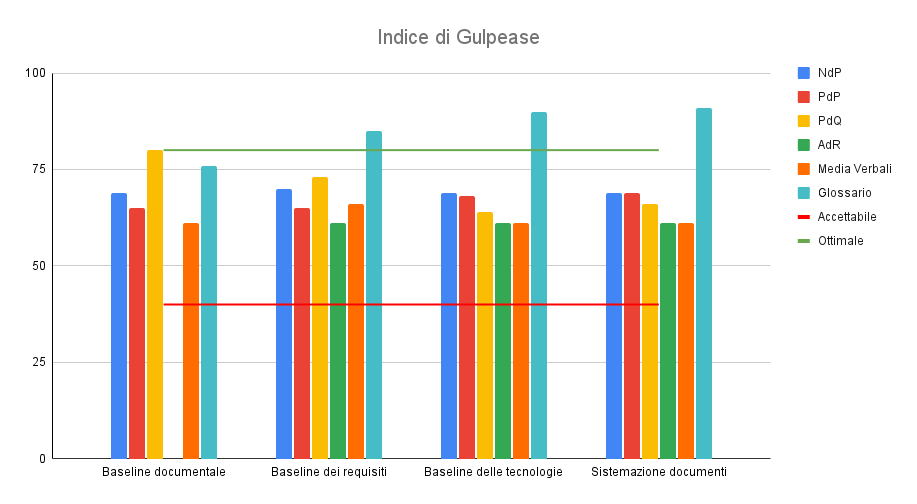
\includegraphics[width=0.8\textwidth, height=0.8\textheight,keepaspectratio]{images/RTB-Indice-di-Gulpease.png}
    \caption{Grafico dell'indice di Gulpease dei documenti nelle varie fasi dell'RTB.}
\end{figure}    

\subsubsection{M15VC - Variazione di Costo}
\begin{figure}[H]
    \centering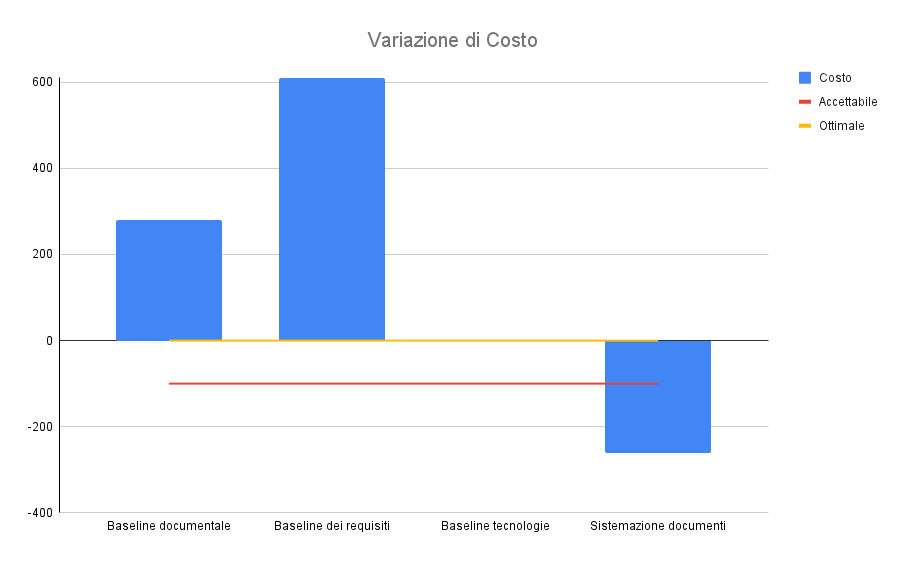
\includegraphics[width=0.8\textwidth, height=0.8\textheight,keepaspectratio]{images/RTB-Variazione-di-Costo.png}
    \caption{Grafico che indica come sono variati i costi rispetto a quelli preventivati nelle varie fasi dell'RTB.}
\end{figure}    

\subsubsection{M16VP - Variazione di Piano}
\begin{figure}[H]
    \centering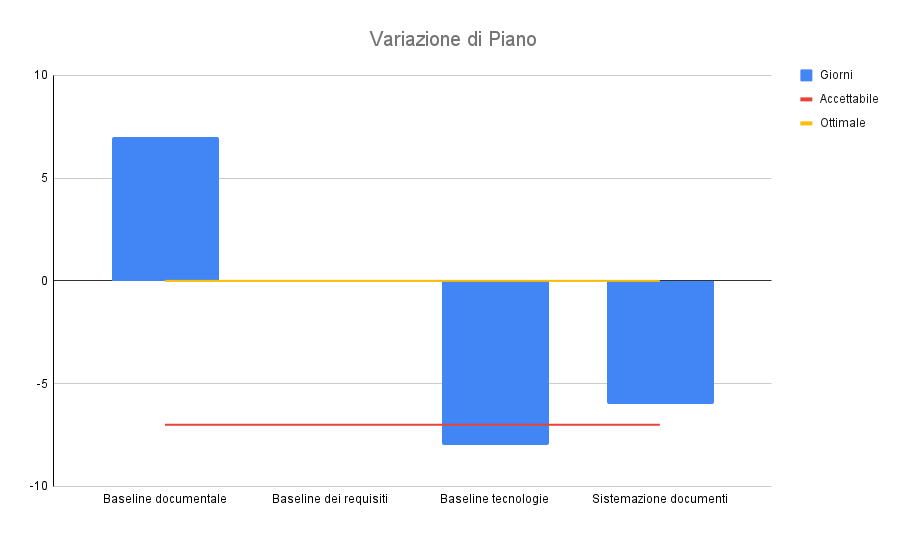
\includegraphics[width=0.8\textwidth, height=0.8\textheight,keepaspectratio]{images/RTB-Variazione-di-Piano.png}
    \caption{Grafico che indica come è variata la pianficazione rispetto al preventivo nelle varie fasi dell'RTB.}
\end{figure}  


\subsection{Macrofase PB}
\subsubsection{M14IG - Indice di Gulpease}
\begin{figure}[H]
    \centering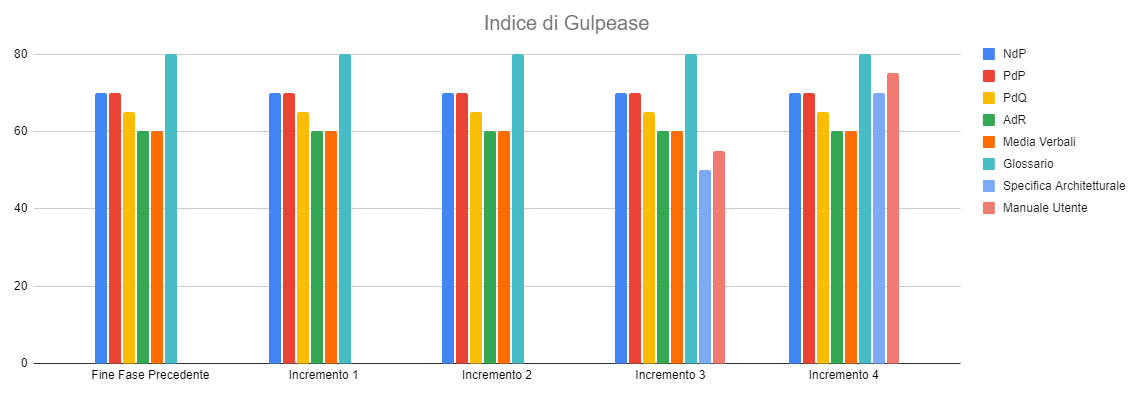
\includegraphics[width=\textwidth, height=\textheight,keepaspectratio]{images/PB-Indice-di-Gulpease.png}
    \caption{Grafico dell'indice di Gulpease dei documenti nelle varie fasi della PB.}
\end{figure}    

\subsubsection{M15VC - Variazione di Costo}
\begin{figure}[H]
    \centering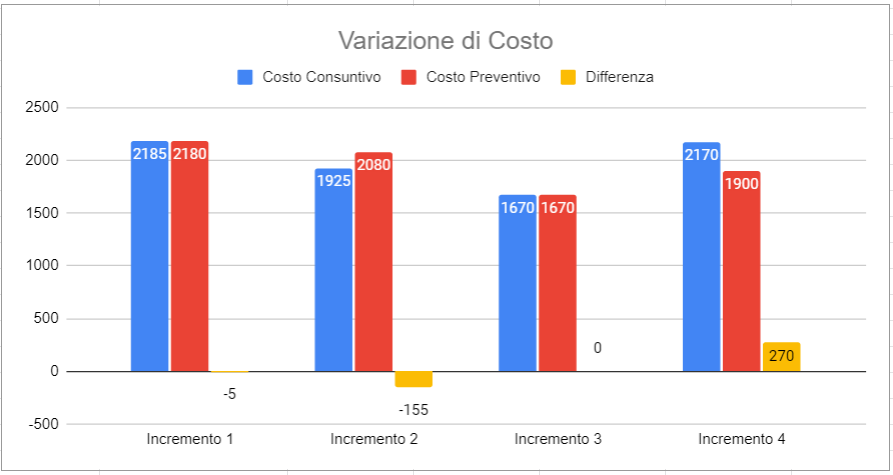
\includegraphics[width=0.8\textwidth, height=0.8\textheight,keepaspectratio]{images/PB-Variazione-di-Costo-2.png}
    \caption{Grafico che indica come sono variati i costi rispetto a quelli preventivati nelle varie fasi della PB.}
\end{figure}    

\subsubsection{M16VP - Variazione di Piano}
\begin{figure}[H]
    \centering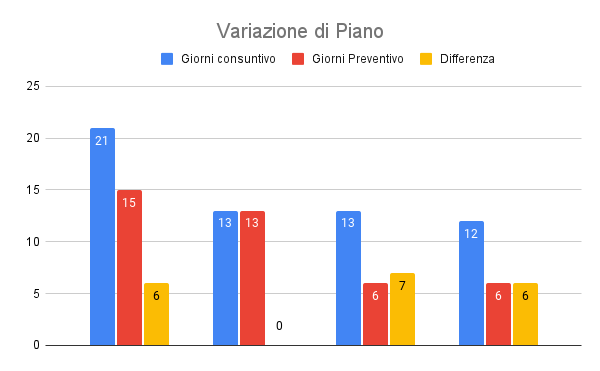
\includegraphics[width=0.8\textwidth, height=0.8\textheight,keepaspectratio]{images/PB-Variazione-di-Piano-3.png}
    \caption{Grafico che indica come è variata la pianificazione rispetto al preventivo nelle varie fasi della PB.}
\end{figure}  

\subsubsection{M8CC - Code Coverage}
\begin{figure}[H]
    \centering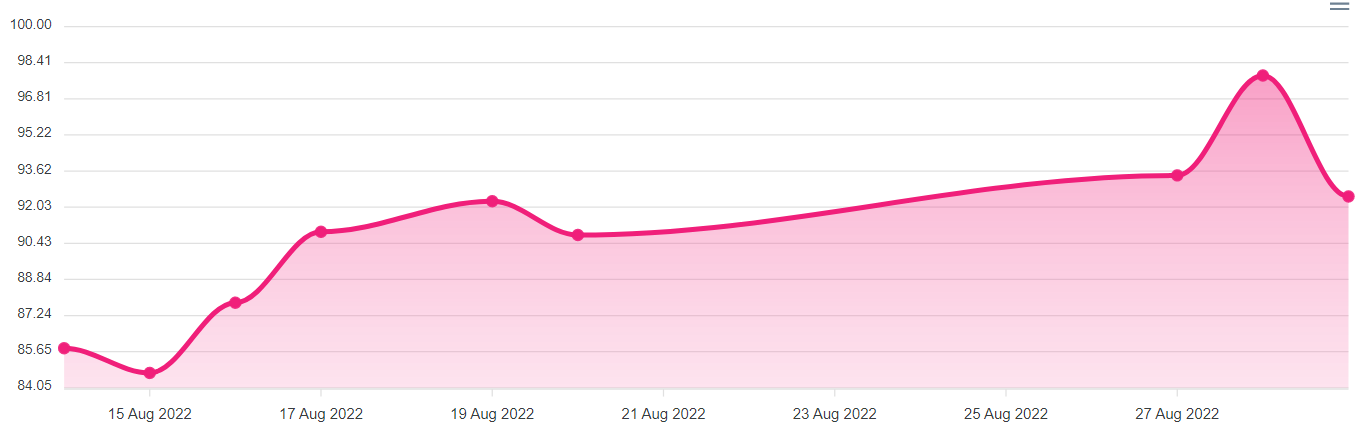
\includegraphics[width=0.8\textwidth, height=0.8\textheight,keepaspectratio]{images/PB-Code-Coverage.png}
    \caption{Grafico che indica come è variata la percentuale di codice coperto da Test nel corso del progetto.}
\end{figure}  

\subsubsection{M1PRR - Percentuale di Requisiti Obbligatori Soddisfatti}
\begin{figure}[H]
    \centering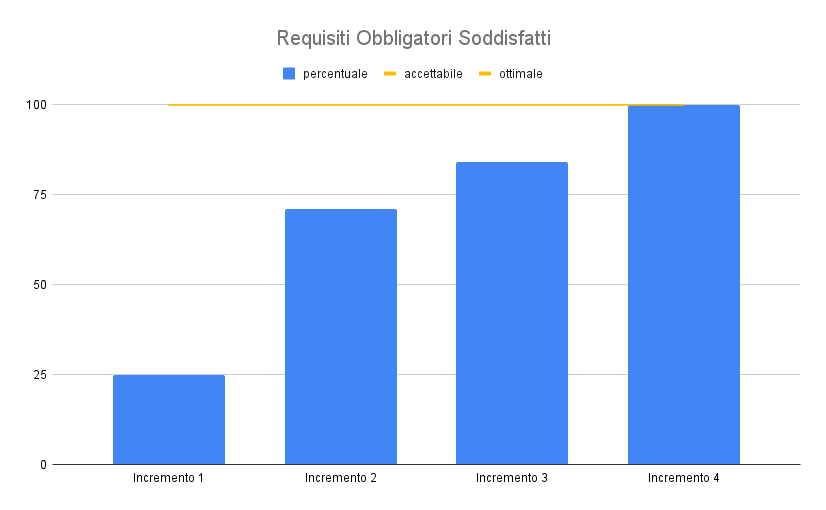
\includegraphics[width=0.8\textwidth, height=0.8\textheight,keepaspectratio]{images/PB-Requisiti-Obbligatori-Soddisfatti.png}
    \caption{Grafico che indica come è variata la percentuale di requisiti obbligatori soddisfatti.}
\end{figure}  

\subsubsection{M2PDR - Percentuale di Requisiti Desiderabili Soddisfatti}
\begin{figure}[H]
    \centering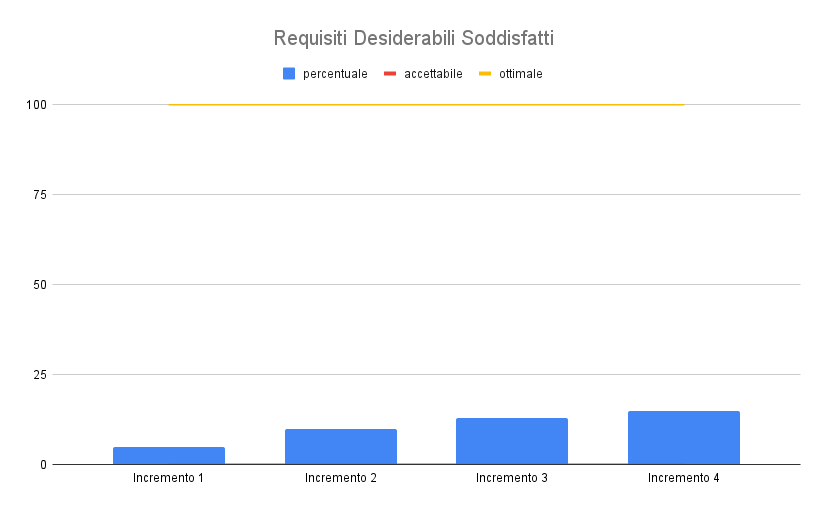
\includegraphics[width=0.8\textwidth, height=0.8\textheight,keepaspectratio]{images/PB-Requisiti-Desiderabili-Soddisfatti.png}
    \caption{Grafico che indica come è variata la percentuale di requisiti desiderabili soddisfatti.}
\end{figure}  